% =============================================================================
%  RELATÓRIO DE ESTÁGIO
%  Licenciatura em Tecnologias da Informação
%  ESTGA - Universidade de Aveiro
%  Ratmir Mukazhanov, n.º 120629
%  Template conforme Guião de Orientação V6 (2026)
% =============================================================================

\documentclass[a4paper,12pt]{report}

% ---------------------------- ENCODING & FONTS --------------------------------
\usepackage[T1]{fontenc}
\usepackage[utf8]{inputenc}
\usepackage{newtxtext,newtxmath}          % Times New Roman

% ---------------------------- LANGUAGE ----------------------------------------
\usepackage[portuguese]{babel}            % Português (novo acordo ortográfico)
\usepackage{csquotes}                     % Recomendado para biblatex

% ---------------------------- GEOMETRY ----------------------------------------
\usepackage[top=2.5cm, bottom=2.5cm, left=2.5cm, right=2.5cm]{geometry}

% ---------------------------- SPACING -----------------------------------------
\usepackage{setspace}
\onehalfspacing                            % Espaçamento entre linhas: 1.5
\setlength{\parindent}{0pt}               % Sem avanço de parágrafos
\setlength{\parskip}{12pt}                % Espaçamento entre parágrafos: 12pt

% ---------------------------- HEADERS & FOOTERS -------------------------------
\usepackage{fancyhdr}

\fancypagestyle{mystyle}{
  \fancyhf{}
  \fancyfoot[R]{\fontsize{10}{12}\selectfont\thepage}
  \renewcommand{\headrulewidth}{0pt}
}

\fancypagestyle{plain}{
  \fancyhf{}
  \fancyfoot[R]{\fontsize{10}{12}\selectfont\thepage}
  \renewcommand{\headrulewidth}{0pt}
}

\pagestyle{mystyle}

% ---------------------------- TITLE FORMATTING --------------------------------
\usepackage{titlesec}

% Título 1 (chapter): 18pt, bold
\titleformat{\chapter}[display]
  {\normalfont\fontsize{18}{22}\selectfont\bfseries}
  {\chaptertitlename\ \thechapter}
  {20pt}
  {\fontsize{18}{22}\selectfont}

% Título 2 (section): 14pt, bold
\titleformat{\section}
  {\normalfont\fontsize{14}{17}\selectfont\bfseries}
  {\thesection}
  {1em}
  {}

% Título 3 (subsection): 13pt, italic
\titleformat{\subsection}
  {\normalfont\fontsize{13}{16}\selectfont\itshape}
  {\thesubsection}
  {1em}
  {}

% ---------------------------- GRAPHICS ----------------------------------------
\usepackage{graphicx}
\usepackage{float}

% ---------------------------- CAPTIONS ----------------------------------------
\usepackage[font=small,labelfont=bf,justification=justified]{caption}

% ---------------------------- TABLES (improved) -------------------------------
\usepackage{array}
\usepackage{booktabs}

% ---------------------------- BIBLIOGRAPHY (IEEE) -----------------------------
\usepackage[style=ieee, sorting=none]{biblatex}
\addbibresource{references.bib}

% ---------------------------- HYPERLINKS --------------------------------------
\usepackage[hidelinks]{hyperref}

% ---------------------------- APPENDICES --------------------------------------
\usepackage[titletoc]{appendix}
\addto\captionsportuguese{%
  \renewcommand{\appendixname}{Anexo}%
  \renewcommand{\appendixtocname}{Anexos}%
  \renewcommand{\appendixpagename}{Anexos}%
}

% ---------------------------- ACRONYMS ----------------------------------------
\usepackage[printonlyused]{acronym}

% ---------------------------- MISC --------------------------------------------
\usepackage{url}
\usepackage{pdfpages}                     % Para incluir PDFs nos anexos

% =============================================================================
\begin{document}

% ===================== CAPA ===================================================
\hypersetup{pageanchor=false}
\thispagestyle{empty}
\begin{center}

  \vspace*{2cm}

  
\includegraphics[width=0.5\textwidth]{images/logoUA.png}

  \vspace{0.5cm}

  {\fontsize{18}{22}\selectfont\bfseries
    Universidade de Aveiro\\
    Escola Superior de Tecnologia e Gestão de Águeda\par}

  \vspace{2cm}

  {\fontsize{20}{24}\selectfont\bfseries
    Título do Relatório de Estágio\par}

  \vspace{1.5cm}

  {\fontsize{14}{17}\selectfont
    Relatório de Estágio\\
    Licenciatura em Tecnologias da Informação\par}

  \vspace{2cm}

  {\fontsize{13}{16}\selectfont
    \textbf{Ratmir Mukazhanov}\\
    N.º Mecanográfico: 120629\par}

  \vspace{1cm}

  {\fontsize{12}{15}\selectfont
    Orientador ESTGA-UA: Prof. Doutor António Augusto Nunes Godinho\\
    Orientador da Entidade de Acolhimento: Bruno Miguel Ferreira Leitão\par}

  \vspace{0.5cm}

  {\fontsize{12}{15}\selectfont
    Entidade de Acolhimento: Devlop -- Leviahub\par}

  \vfill

  {\fontsize{12}{15}\selectfont
    Águeda, junho de 2026\par}

\end{center}

% ===================== FOLHA EM BRANCO ========================================
\newpage
\thispagestyle{empty}
\phantom{}
\newpage

% ===================== FOLHA DE ROSTO =========================================
\thispagestyle{empty}
\begin{center}

  \vspace*{2cm}

  
\includegraphics[width=0.5\textwidth]{images/logoUA.png}

  \vspace{0.5cm}

  {\fontsize{18}{22}\selectfont\bfseries
    Universidade de Aveiro\\
    Escola Superior de Tecnologia e Gestão de Águeda\par}

  \vspace{2cm}

  {\fontsize{20}{24}\selectfont\bfseries
    Título do Relatório de Estágio\par}

  \vspace{1.5cm}

  {\fontsize{14}{17}\selectfont
    Relatório de Estágio\\
    Licenciatura em Tecnologias da Informação\par}

  \vspace{2cm}

  {\fontsize{13}{16}\selectfont
    \textbf{Ratmir Mukazhanov}\\
    N.º Mecanográfico: 120629\par}

  \vspace{1cm}

  {\fontsize{12}{15}\selectfont
    Orientador ESTGA-UA: Prof. Doutor António Augusto Nunes Godinho\\
    Orientador da Entidade de Acolhimento: Bruno Miguel Ferreira Leitão\par}

  \vspace{0.5cm}

  {\fontsize{12}{15}\selectfont
    Entidade de Acolhimento: Devlop -- Leviahub\par}

  \vfill

  {\fontsize{12}{15}\selectfont
    Águeda, junho de 2026\par}

\end{center}

% ===================== NUMERAÇÃO ROMANA (PRELIMINARES) ========================
\newpage
\hypersetup{pageanchor=true}
\pagenumbering{roman}
\setcounter{page}{4}

% ===================== AGRADECIMENTOS (FACULTATIVO) ===========================
% --- Descomentar se pretender incluir agradecimentos ---
% \chapter*{Agradecimentos}
% \addcontentsline{toc}{chapter}{Agradecimentos}
%
% Texto dos agradecimentos...
%
% \newpage

% ===================== RESUMO =================================================
\chapter*{Resumo}
\addcontentsline{toc}{chapter}{Resumo}

Texto do resumo em português (máximo de 300 palavras).

\vspace{1cm}
\noindent\textbf{Palavras-chave:} palavra-chave 1; palavra-chave 2; palavra-chave 3; palavra-chave 4; palavra-chave 5; palavra-chave 6.

\newpage

% ===================== ABSTRACT ===============================================
\chapter*{Abstract}
\addcontentsline{toc}{chapter}{Abstract}

Abstract text in English (maximum 300 words).

\vspace{1cm}
\noindent\textbf{Keywords:} keyword 1; keyword 2; keyword 3; keyword 4; keyword 5; keyword 6.

\newpage

% ===================== ÍNDICE =================================================
\tableofcontents
\newpage

\listoffigures
\addcontentsline{toc}{chapter}{\listfigurename}
\newpage

\listoftables
\addcontentsline{toc}{chapter}{\listtablename}

% ===================== LISTA DE SIGLAS E ABREVIATURAS (FACULTATIVO) ===========
% --- Descomentar se pretender incluir lista de siglas ---
% \newpage
% \chapter*{Lista de Siglas e Abreviaturas}
% \addcontentsline{toc}{chapter}{Lista de Siglas e Abreviaturas}
%
% \begin{acronym}
%   \acro{ESTGA}{Escola Superior de Tecnologia e Gestão de Águeda}
%   \acro{UA}{Universidade de Aveiro}
%   \acro{TI}{Tecnologias da Informação}
%   \acro{EA}{Entidade de Acolhimento}
%   \acro{PIT}{Plano Individual de Trabalho}
% \end{acronym}
%
% \newpage

% ===================== NUMERAÇÃO ÁRABE (CORPO DO RELATÓRIO) ===================
\pagenumbering{arabic}
\setcounter{page}{1}

% ===================== CAPÍTULO 1 - INTRODUÇÃO ================================
\chapter{Introdução}

% --- Apresentação do tema e da Entidade de Acolhimento ---
\section{Enquadramento}

Texto de apresentação do tema do estágio/projeto e da Entidade de Acolhimento
(EA). Descrever sucintamente a empresa/instituição onde o estágio/projeto foi
realizado, a sua área de atuação e o contexto em que o trabalho se insere.

% --- Objetivos ---
\section{Objetivos}

\subsection{Objetivos gerais}

Descrição do(s) objetivo(s) geral(ais) do estágio/projeto.

\subsection{Objetivos específicos}

Enumeração e descrição dos objetivos específicos que se pretendem alcançar com
o trabalho realizado.

% --- Metodologia ---
\section{Metodologia}

Indicação da metodologia de trabalho adotada durante o estágio/projeto.

% --- Estrutura do relatório ---
\section{Estrutura do Relatório}

Breve descrição da estrutura interna do relatório, indicando o conteúdo de cada
capítulo.

% ===================== CAPÍTULO 2 - PLANEAMENTO DO TRABALHO ===================
\chapter{Planeamento do Trabalho}

\section{Plano de Trabalho}

Identificação e descrição das atividades previstas para a realização do
estágio/projeto, incluindo a calendarização definida no Plano Individual de
Trabalho (PIT).

% --- Exemplo de tabela ---
% \begin{table}[h]
%   \centering
%   \caption{Planeamento das atividades do estágio/projeto}
%   \label{tab:planeamento}
%   \begin{tabular}{|c|c|c|c|}
%     \hline
%     \textbf{ID} & \textbf{Atividade} & \textbf{Data de Início} & \textbf{Data de Fim} \\
%     \hline
%     A1 & Atividade 1 & mês/ano & mês/ano \\
%     \hline
%     A2 & Atividade 2 & mês/ano & mês/ano \\
%     \hline
%   \end{tabular}
% \end{table}
%
% A Tabela~\ref{tab:planeamento} apresenta o plano de trabalho previsto.

% ===================== CAPÍTULO 3 - ATIVIDADES DESENVOLVIDAS ==================
\chapter{Descrição das Atividades Desenvolvidas}

\section{Atividade 1}

Descrição e análise detalhada da primeira atividade desenvolvida no âmbito do
estágio/projeto.

\subsection{Tarefas realizadas}

Descrição das tarefas concretas.

\subsection{Resultados obtidos}

Apresentação e discussão dos resultados.

\section{Atividade 2}

Descrição e análise detalhada da segunda atividade.

% --- Exemplo de figura ---
% \begin{figure}[h]
%   \centering
%   % \includegraphics[width=0.8\textwidth]{images/exemplo.png}
%   \caption{Legenda da figura.}
%   \label{fig:exemplo}
% \end{figure}
%
% A Figura~\ref{fig:exemplo} ilustra o processo descrito.

% ===================== CAPÍTULO 4 - ANÁLISE DE RESULTADOS =====================
\chapter{Análise de Resultados}

\section{Cumprimento dos Objetivos}

Análise do cumprimento dos objetivos gerais e específicos definidos inicialmente
para o estágio/projeto.

\section{Discussão}

Discussão dos principais resultados obtidos, dificuldades encontradas e
soluções adotadas.

% ===================== CAPÍTULO 5 - CONCLUSÕES ================================
\chapter{Conclusões}

\section{Reflexão Crítica}

Reflexão crítica sobre o trabalho de estágio/projeto realizado, incidindo sobre
os seguintes aspetos:

\begin{itemize}
  \item Atividades desenvolvidas
  \item Estratégias de trabalho adotadas
  \item Tecnologias utilizadas
  \item Planeamento previsto e o efetivamente executado
  \item Sugestões que possam colmatar eventuais lacunas do trabalho realizado
\end{itemize}

\section{Trabalho Futuro}

Sugestões de melhorias e desenvolvimentos futuros que possam dar continuidade
ao trabalho realizado.

% ===================== BIBLIOGRAFIA ===========================================
\printbibliography

% ===================== ANEXOS =================================================
\begin{appendices}
\renewcommand{\thefigure}{\arabic{figure}}
\setcounter{figure}{0}

% --- Anexo 1: PIT (2 anexos) ---
\chapter{Plano Individual de Trabalho (PIT)}

\begin{figure}[H]
  \centering
  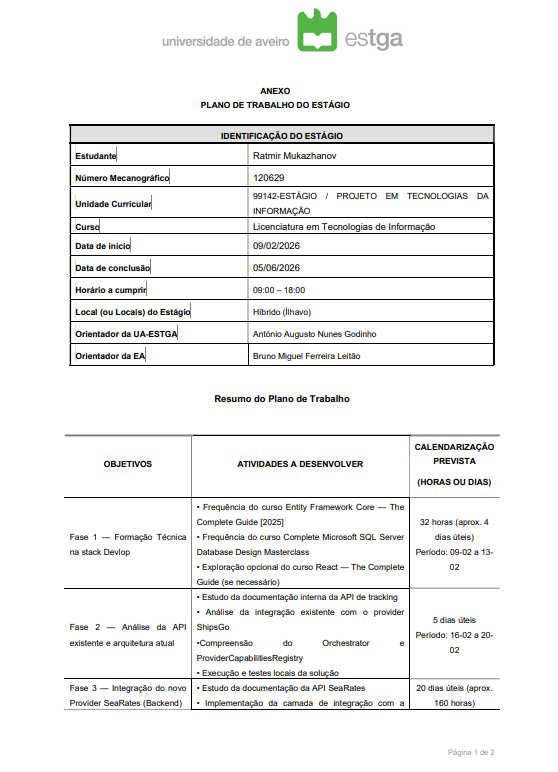
\includegraphics[width=\textwidth]{images/image3.png}
  \caption{Plano do estágio, página 1}
  \label{fig:pit-pag1}
\end{figure}

\begin{figure}[H]
  \centering
  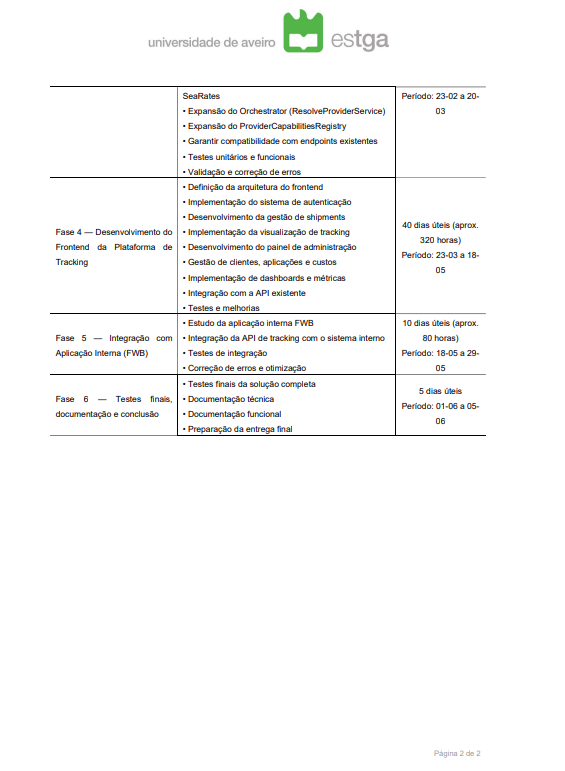
\includegraphics[width=\textwidth]{images/image4.png}
  \caption{Plano do estágio, página 2}
  \label{fig:pit-pag2}
\end{figure}

% --- Anexo 2: Descrição Técnica de Tarefas (5 anexos) ---
\chapter{Descrição Técnica de Tarefas}

\begin{figure}[H]
  \centering
  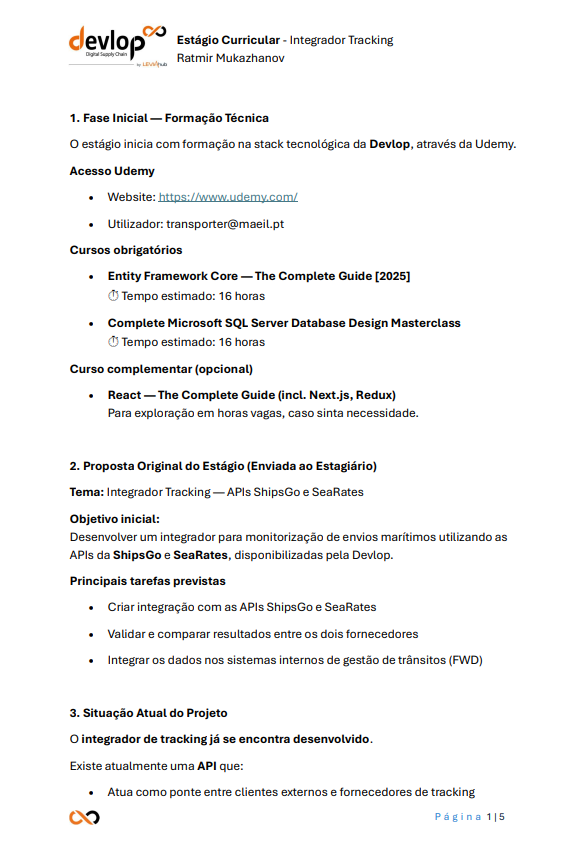
\includegraphics[width=\textwidth]{images/image5.png}
  \caption{Descrição de tarefas, página 1}
  \label{fig:tarefas-pag1}
\end{figure}

\begin{figure}[H]
  \centering
  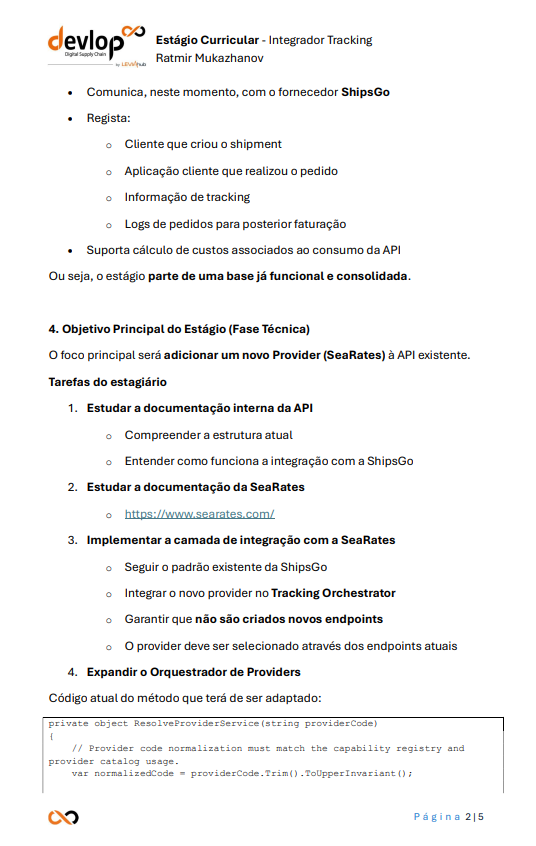
\includegraphics[width=\textwidth]{images/image6.png}
  \caption{Descrição de tarefas, página 2}
  \label{fig:tarefas-pag2}
\end{figure}

\begin{figure}[H]
  \centering
  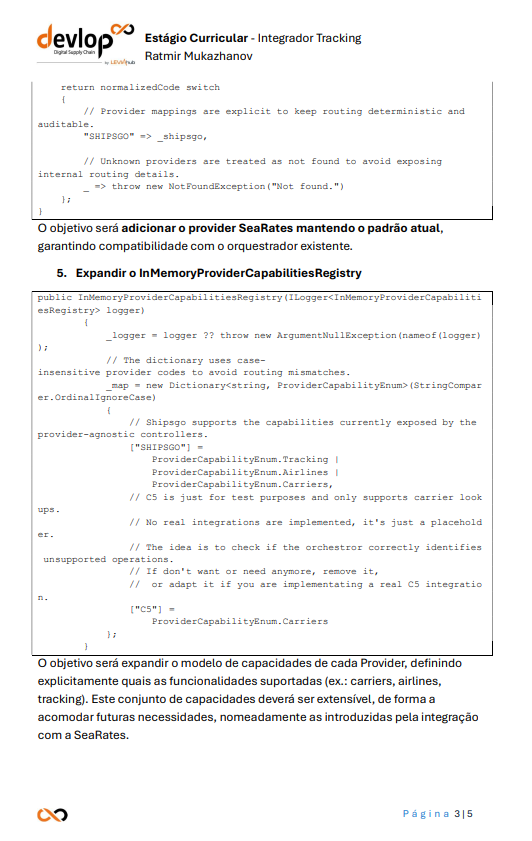
\includegraphics[width=\textwidth]{images/image7.png}
  \caption{Descrição de tarefas, página 3}
  \label{fig:tarefas-pag3}
\end{figure}

\begin{figure}[H]
  \centering
  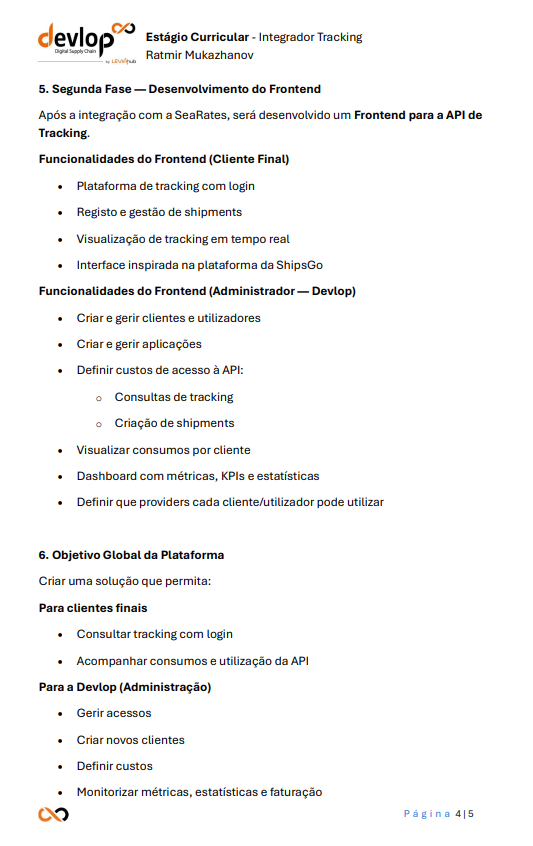
\includegraphics[width=\textwidth]{images/image8.png}
  \caption{Descrição de tarefas, página 4}
  \label{fig:tarefas-pag4}
\end{figure}

\begin{figure}[H]
  \centering
  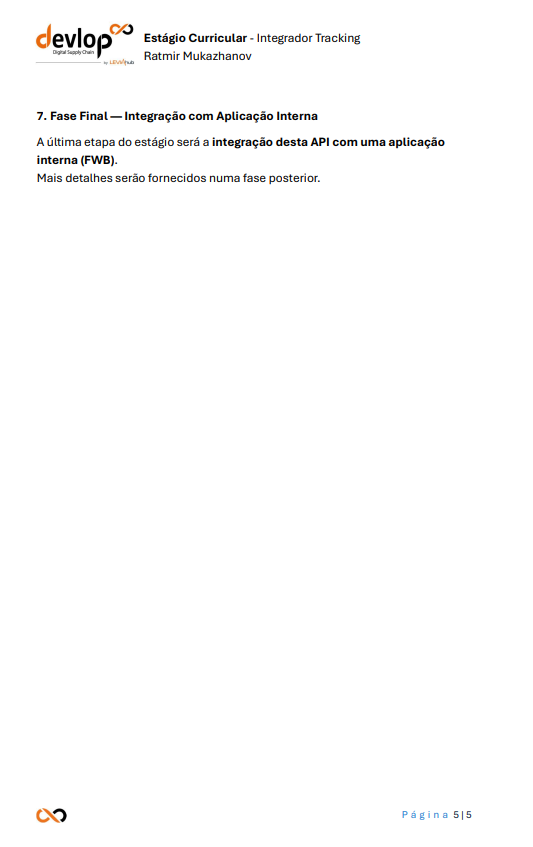
\includegraphics[width=\textwidth]{images/image9.png}
  \caption{Descrição de tarefas, página 5}
  \label{fig:tarefas-pag5}
\end{figure}

% --- Anexo 3: Diagrama de Gantt (1 anexo) ---
\chapter{Diagrama de Gantt}

\begin{figure}[H]
  \centering
  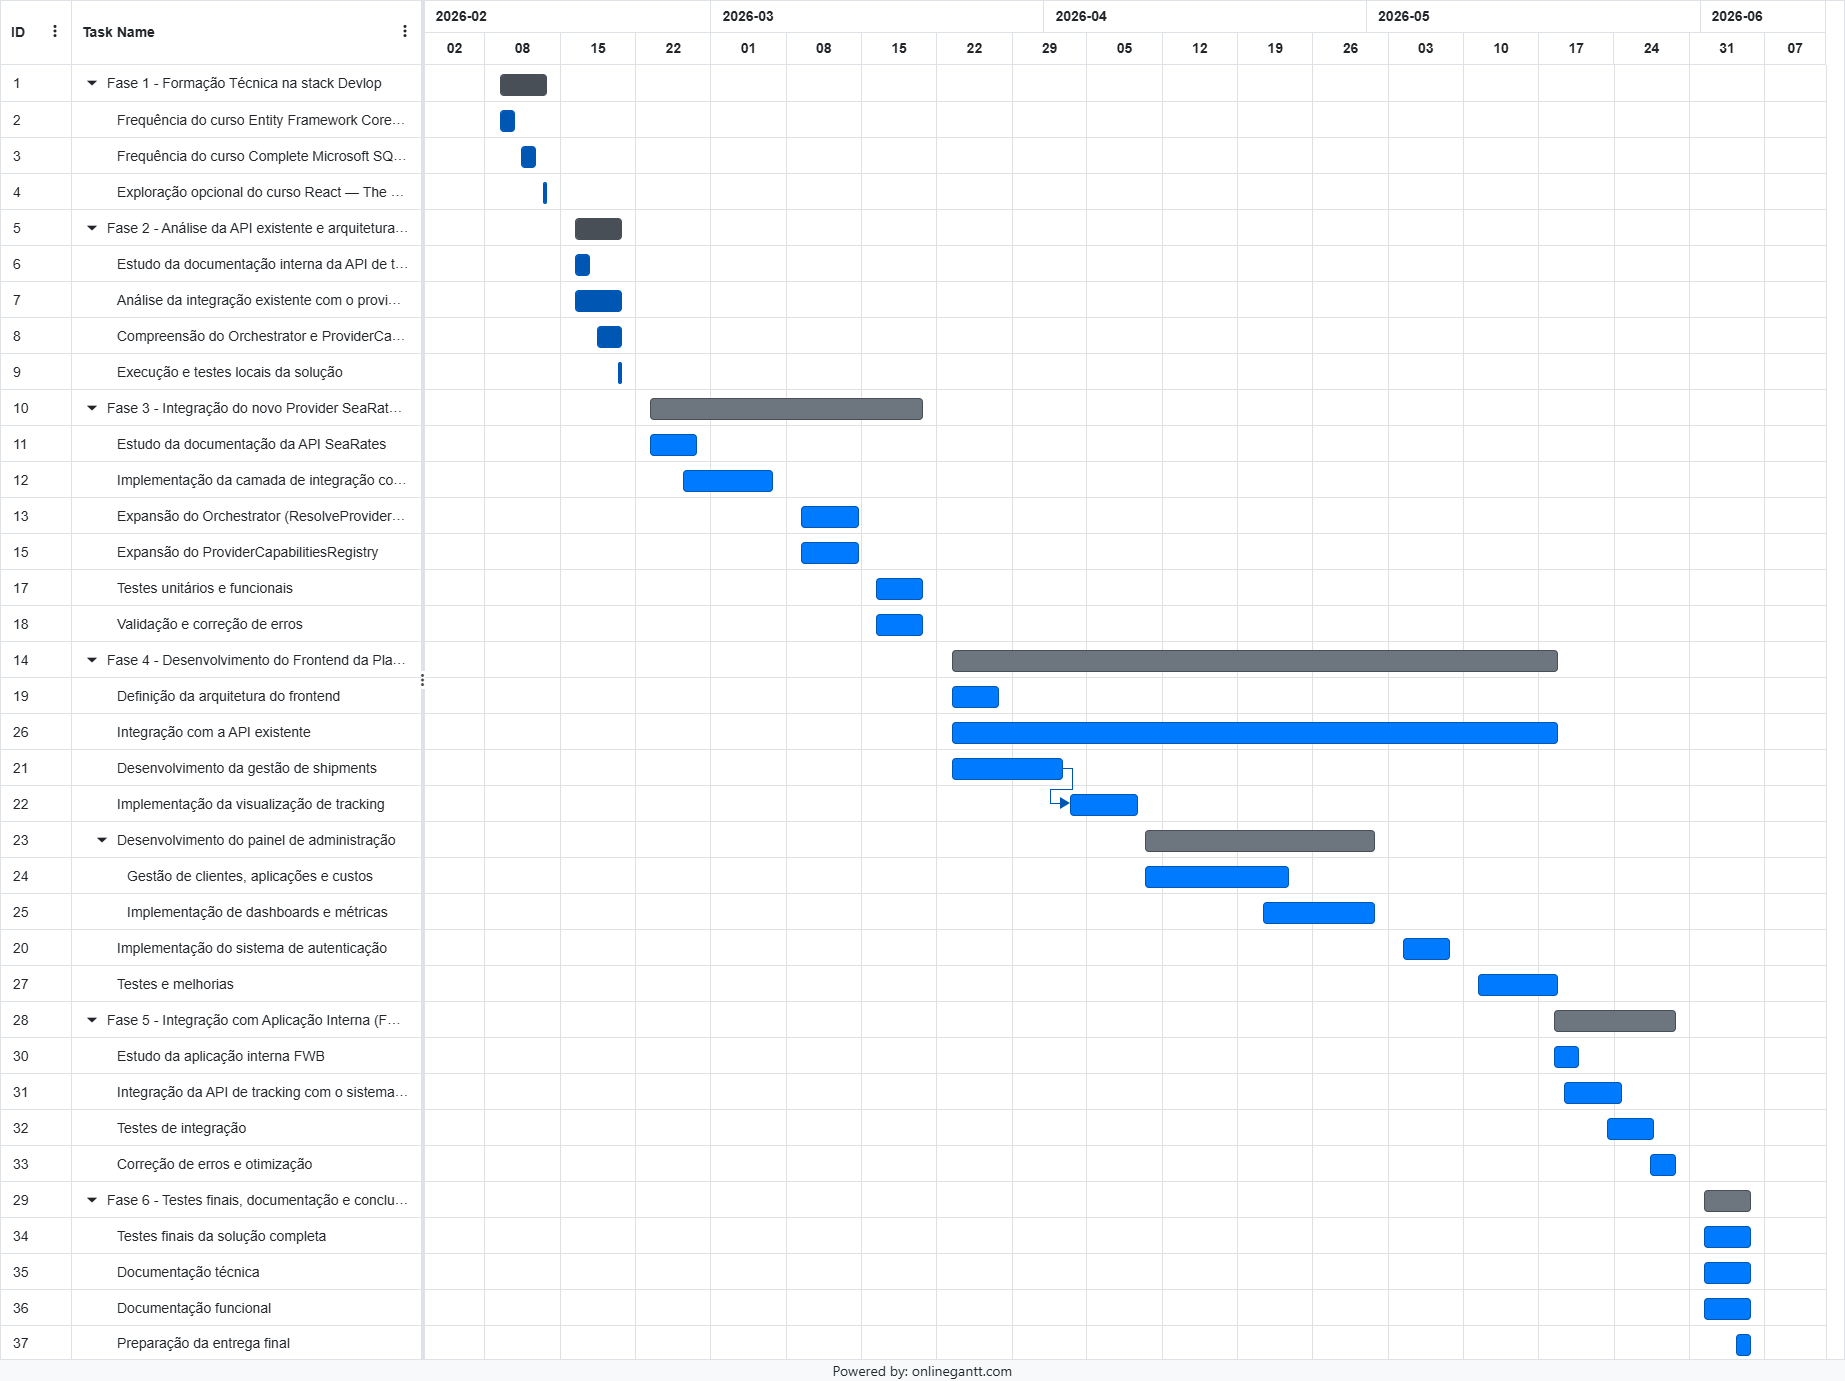
\includegraphics[width=\textwidth]{images/image10.png}
  \caption{Diagrama de Gantt da calendarização prevista}
  \label{fig:gantt}
\end{figure}

% --- Anexo 4: Horário Letivo e Disponibilidade (1 anexo) ---
\chapter{Horário Letivo e Disponibilidade}

\begin{figure}[H]
  \centering
  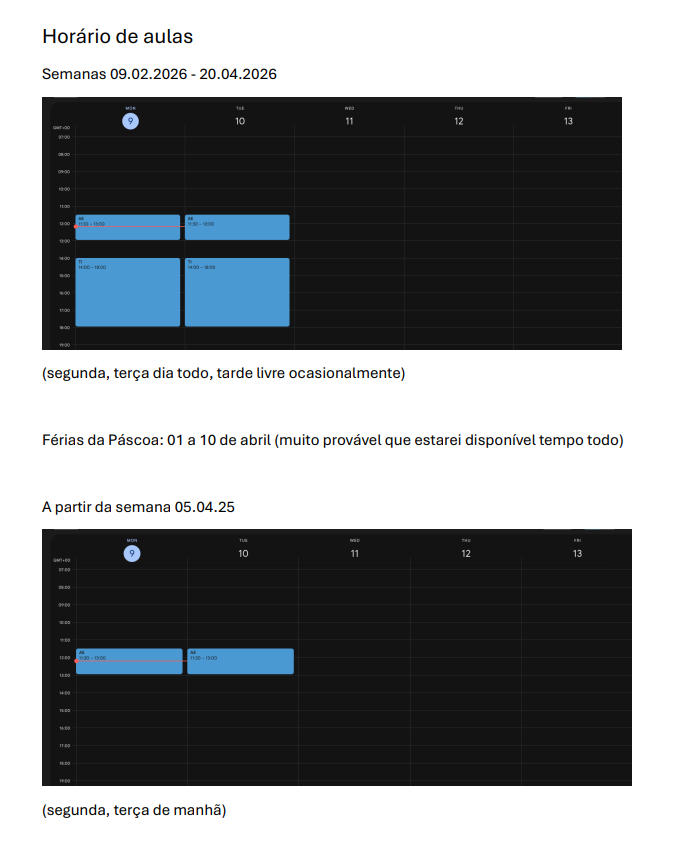
\includegraphics[width=\textwidth]{images/image11.png}
  \caption{Horário Letivo e Disponibilidade}
  \label{fig:horario}
\end{figure}

% --- Anexo 5: Proposta de Métricas Tracking API (3 anexos) ---
\chapter{Proposta de Métricas \textit{Tracking API}}

\begin{figure}[H]
  \centering
  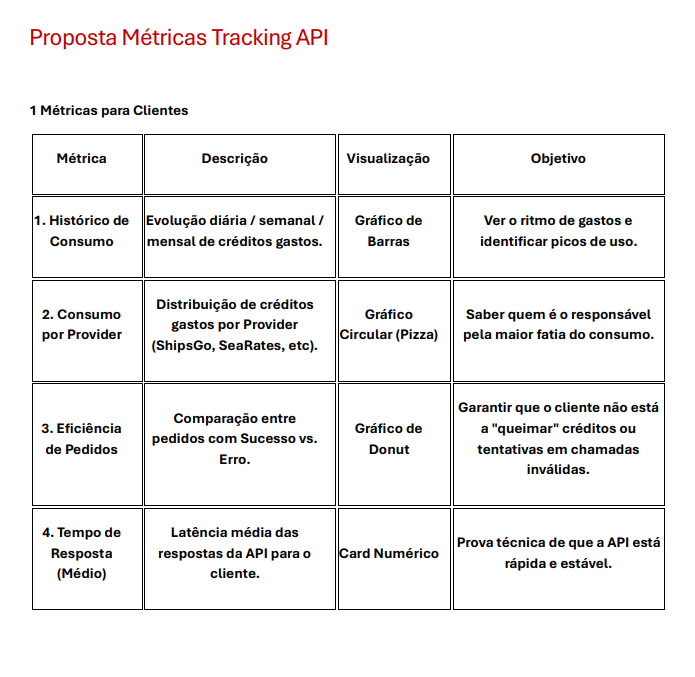
\includegraphics[width=\textwidth]{images/image12.png}
  \caption{Proposta de Métricas \textit{Tracking API}, página 1}
  \label{fig:metricas-pag1}
\end{figure}

\begin{figure}[H]
  \centering
  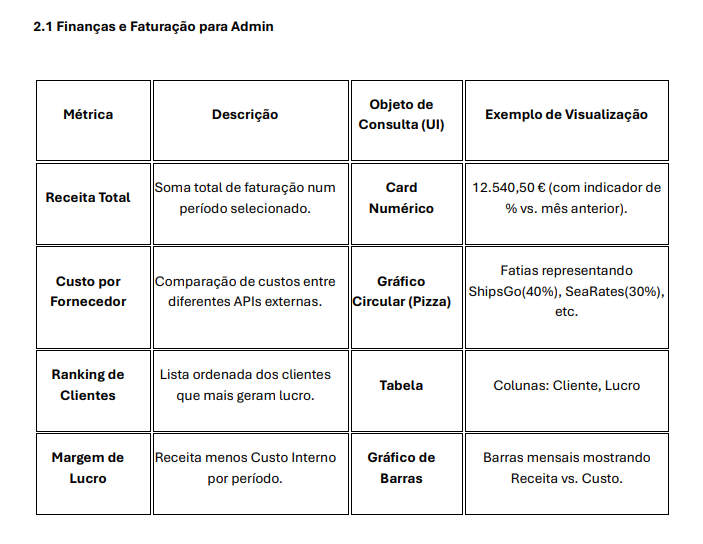
\includegraphics[width=\textwidth]{images/image13.png}
  \caption{Proposta de Métricas \textit{Tracking API}, página 2}
  \label{fig:metricas-pag2}
\end{figure}

\begin{figure}[H]
  \centering
  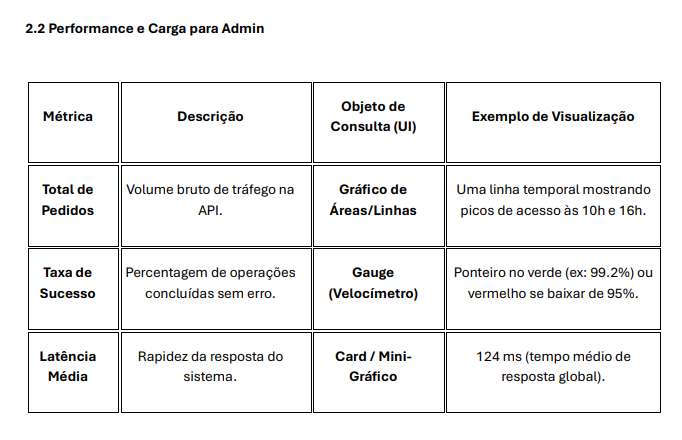
\includegraphics[width=\textwidth]{images/image14.png}
  \caption{Proposta de Métricas \textit{Tracking API}, página 3}
  \label{fig:metricas-pag3}
\end{figure}

% --- Anexo 6: Preparação do Ambiente 4GL (2 anexos) ---
\chapter{Preparação do Ambiente 4GL}

\begin{figure}[H]
  \centering
  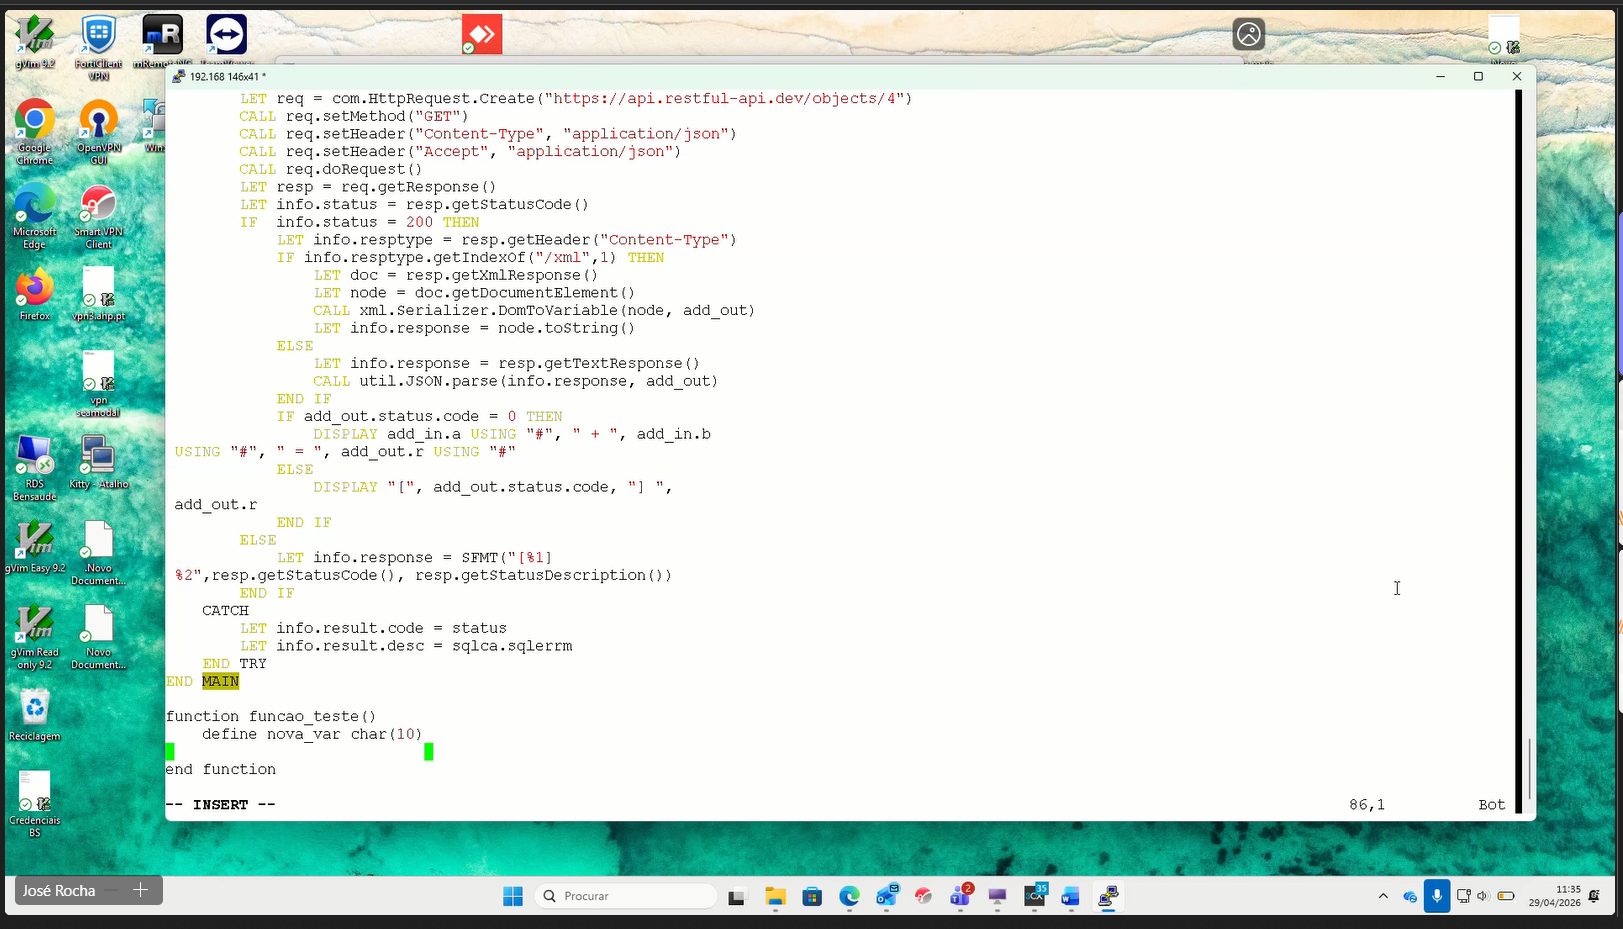
\includegraphics[width=\textwidth]{images/image15.png}
  \caption{Ambiente exemplo de desenvolvimento 4GL}
  \label{fig:4gl-exemplo}
\end{figure}

\begin{figure}[H]
  \centering
  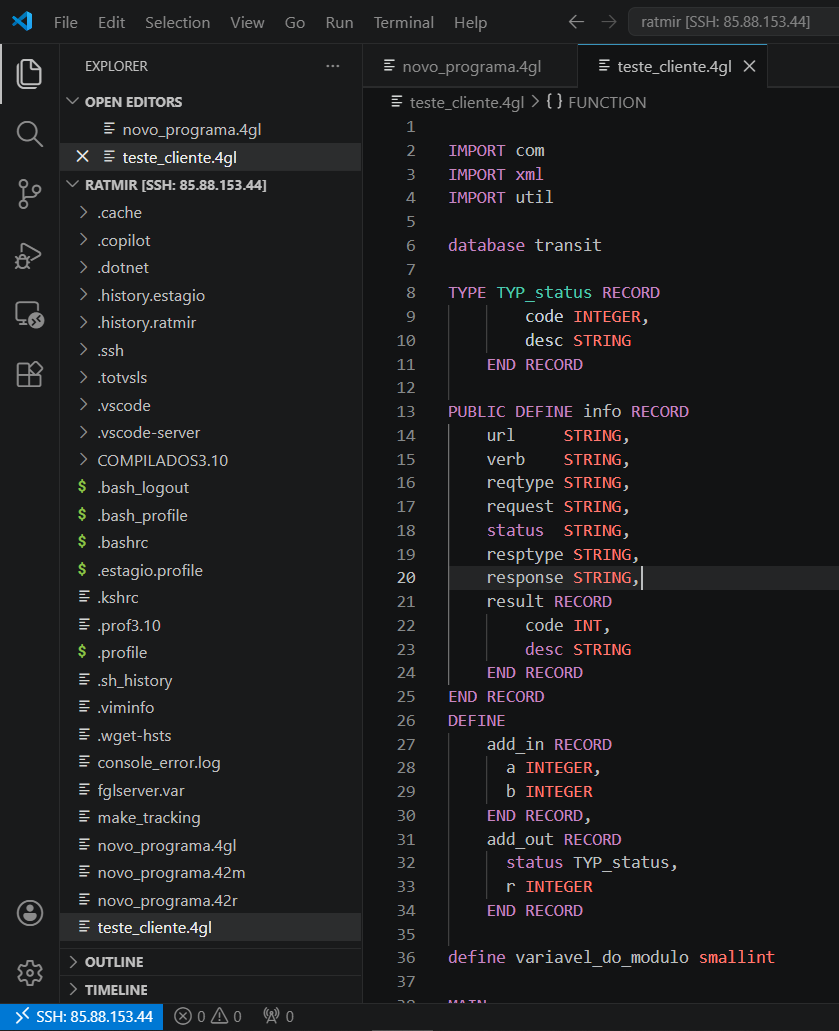
\includegraphics[width=\textwidth]{images/image16.png}
  \caption{Ambiente de desenvolvimento 4GL configurado}
  \label{fig:4gl-configurado}
\end{figure}

% --- Anexo 7: Capturas de Ecrã da Solução (8 anexos) ---
\chapter{Capturas de Ecrã da Solução}

\begin{figure}[H]
  \centering
  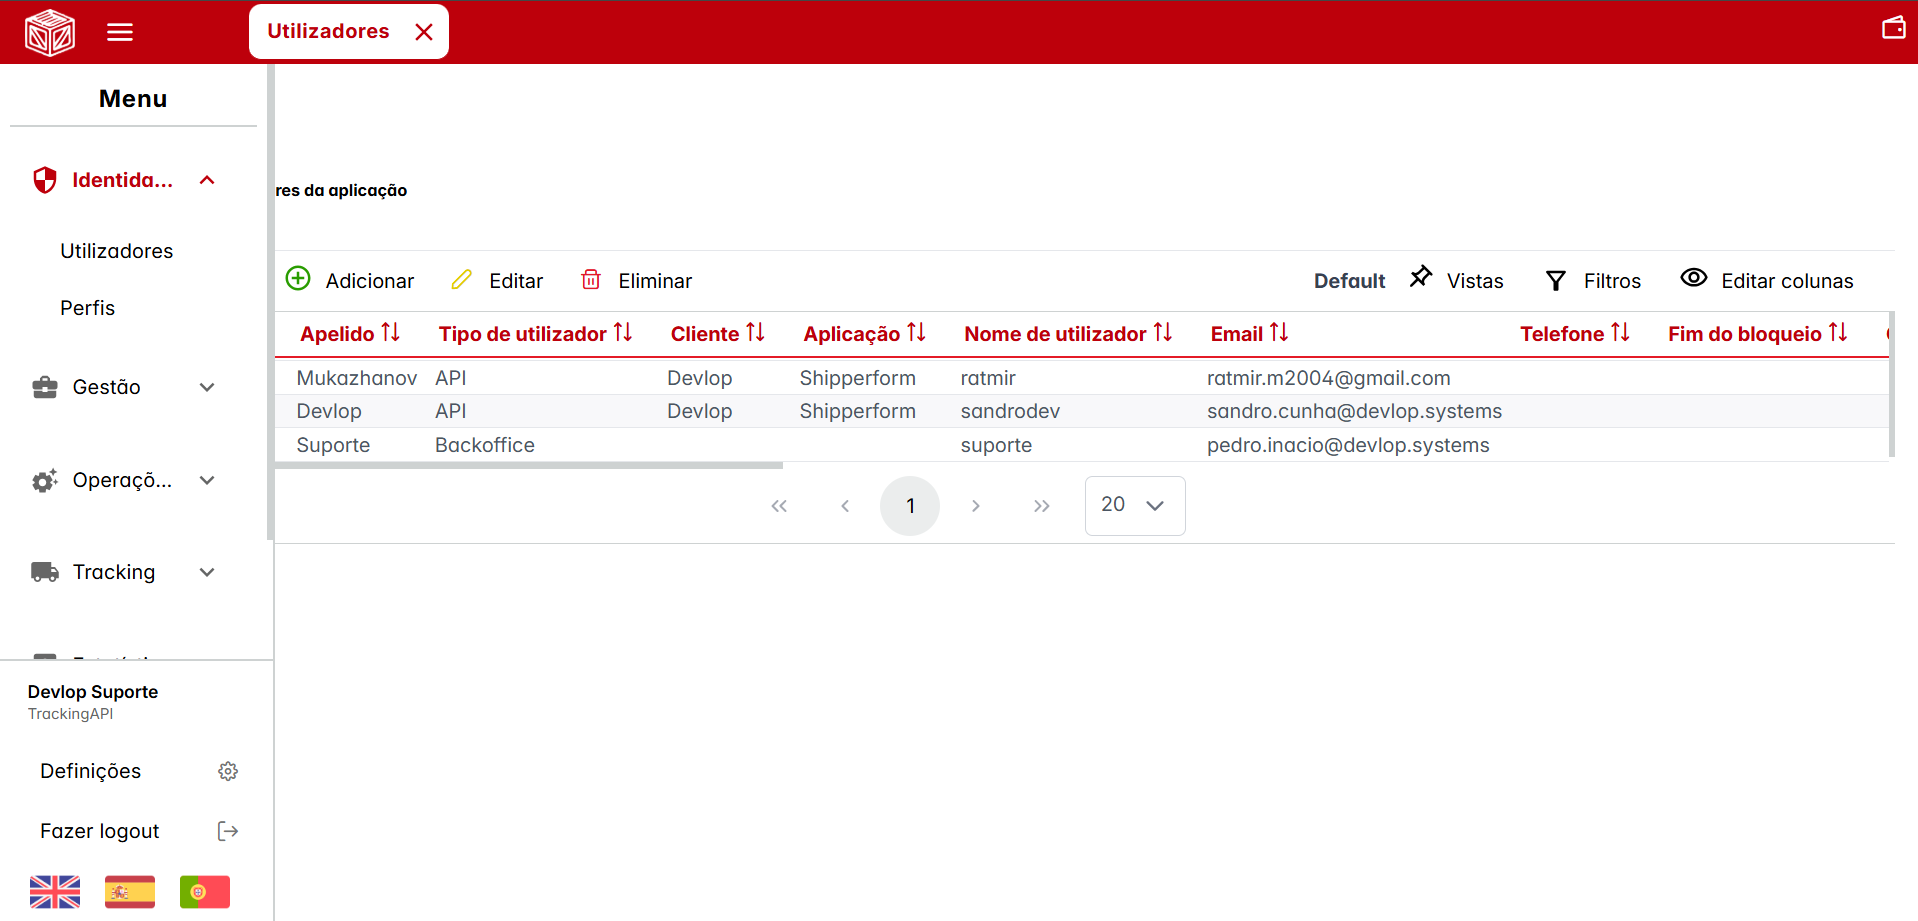
\includegraphics[width=\textwidth]{images/image17.png}
  \caption{Menu lateral e gestão de utilizadores}
  \label{fig:solucao-menu}
\end{figure}

\begin{figure}[H]
  \centering
  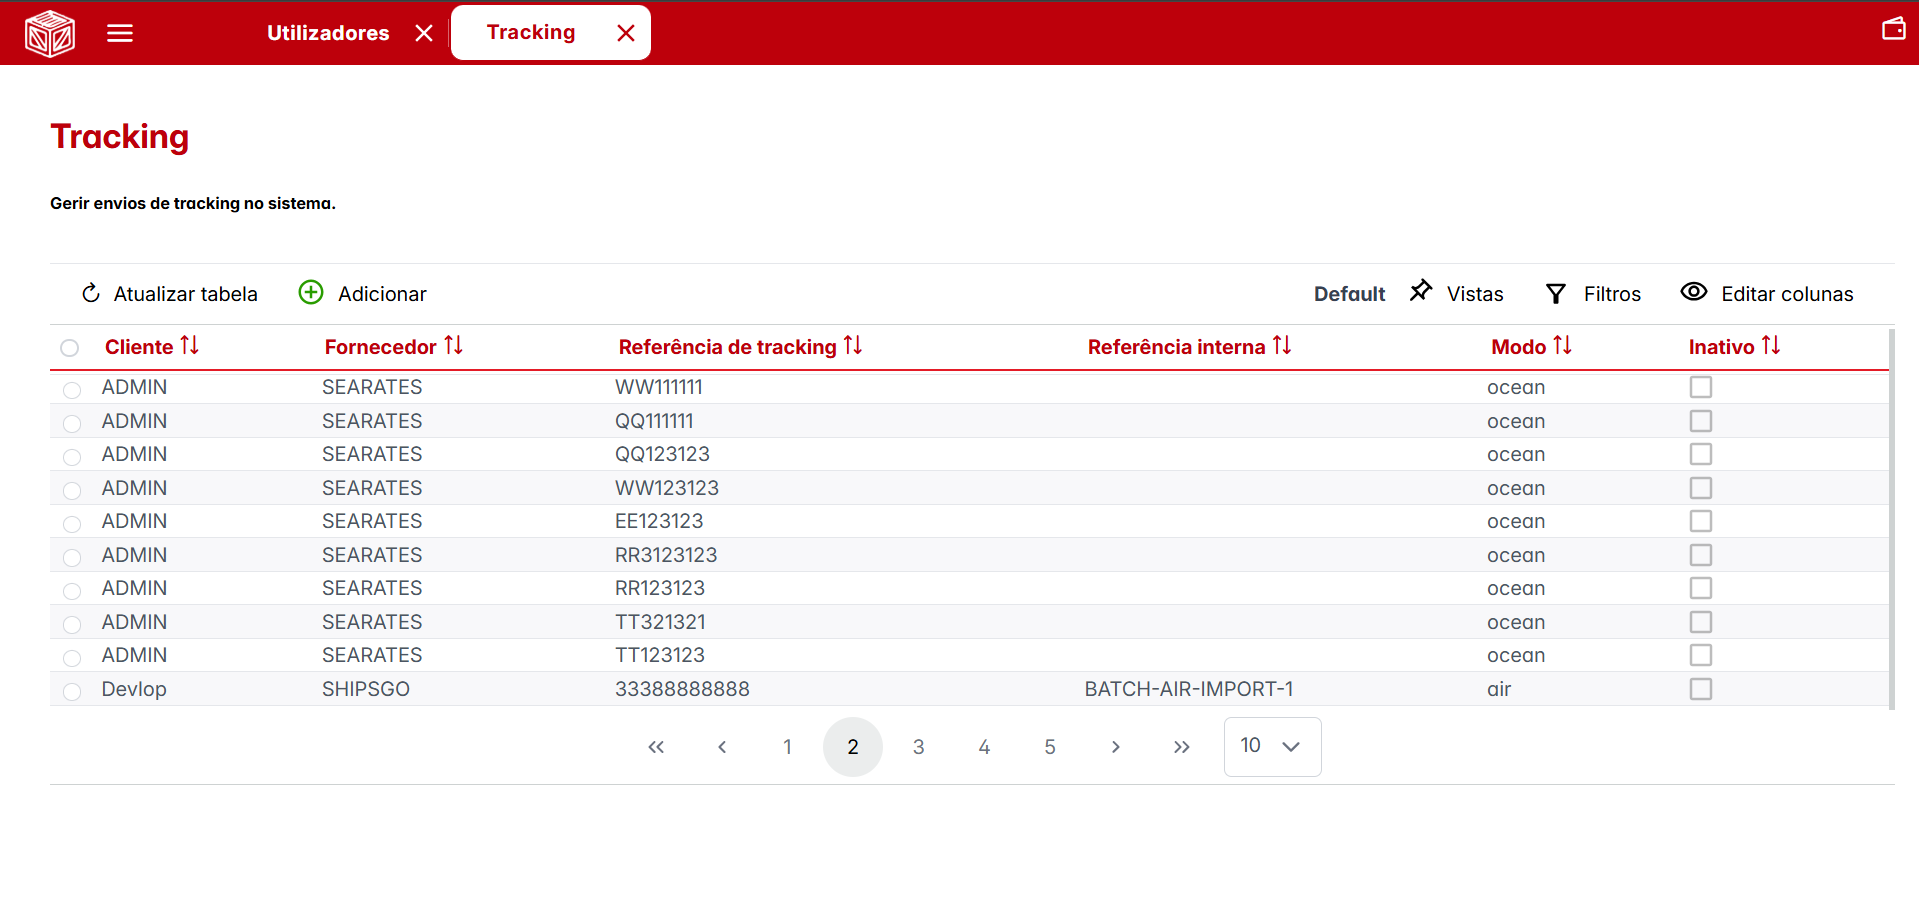
\includegraphics[width=\textwidth]{images/image18.png}
  \caption{Listagem de envios}
  \label{fig:solucao-envios}
\end{figure}

\begin{figure}[H]
  \centering
  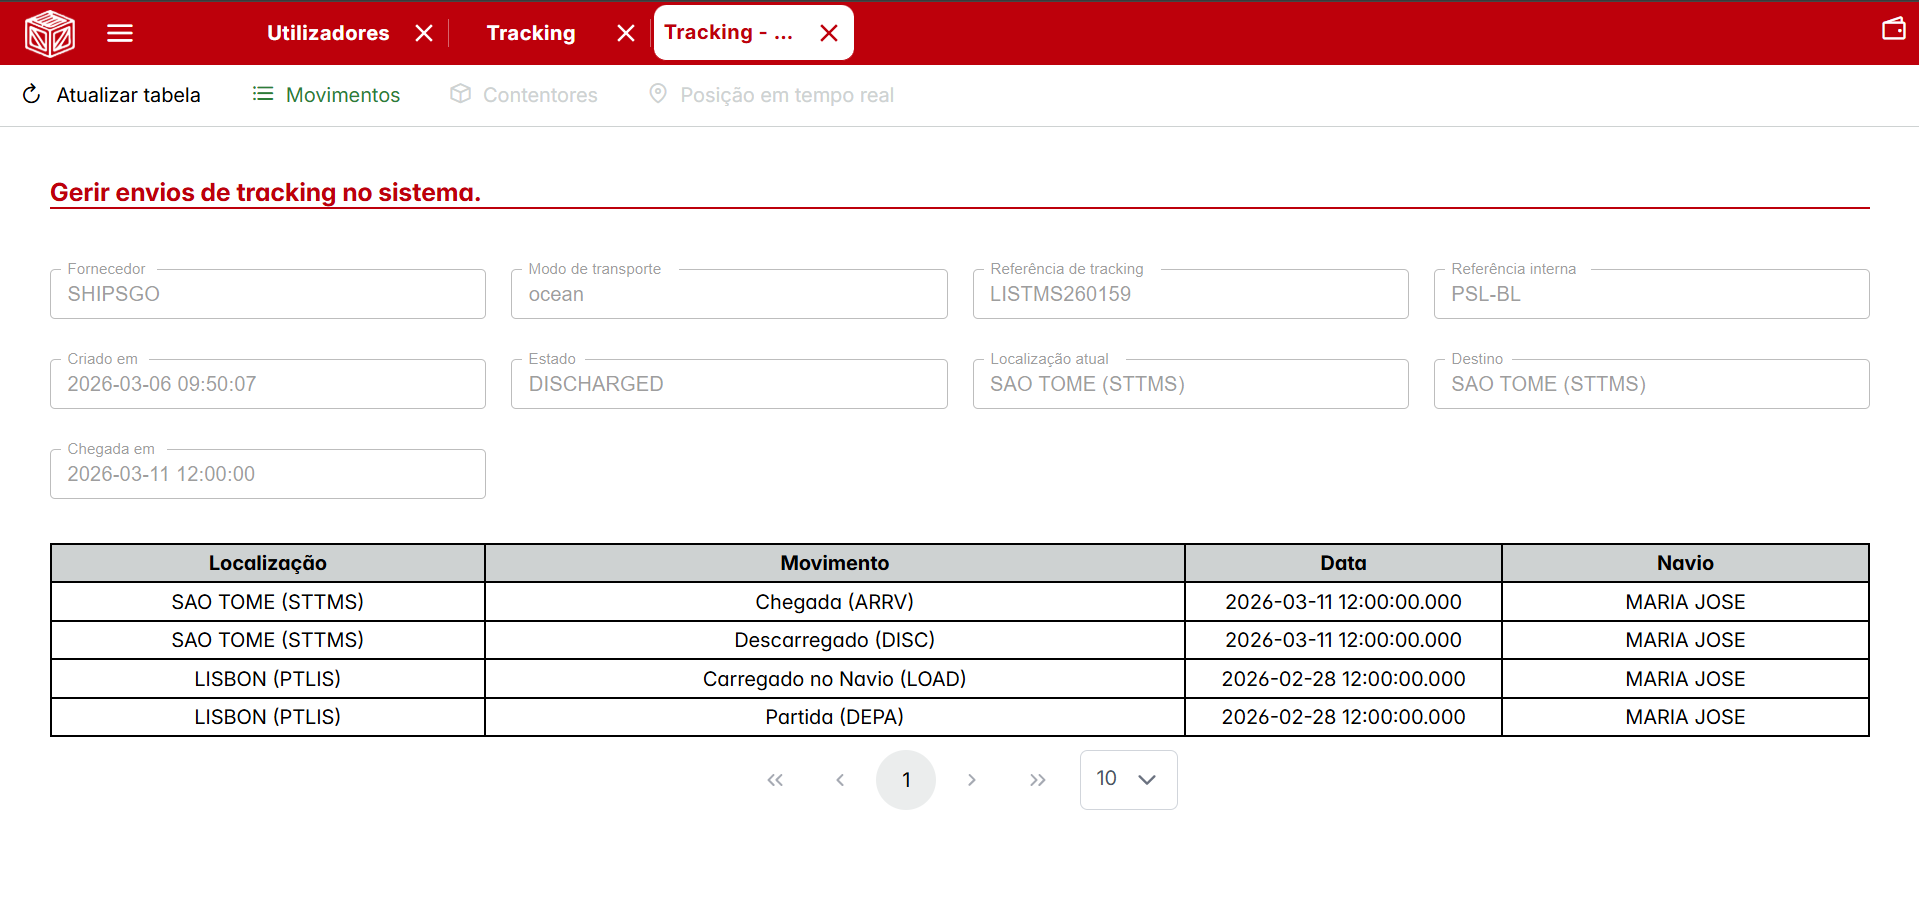
\includegraphics[width=\textwidth]{images/image19.png}
  \caption{Movimentos do envio}
  \label{fig:solucao-movimentos}
\end{figure}

\begin{figure}[H]
  \centering
  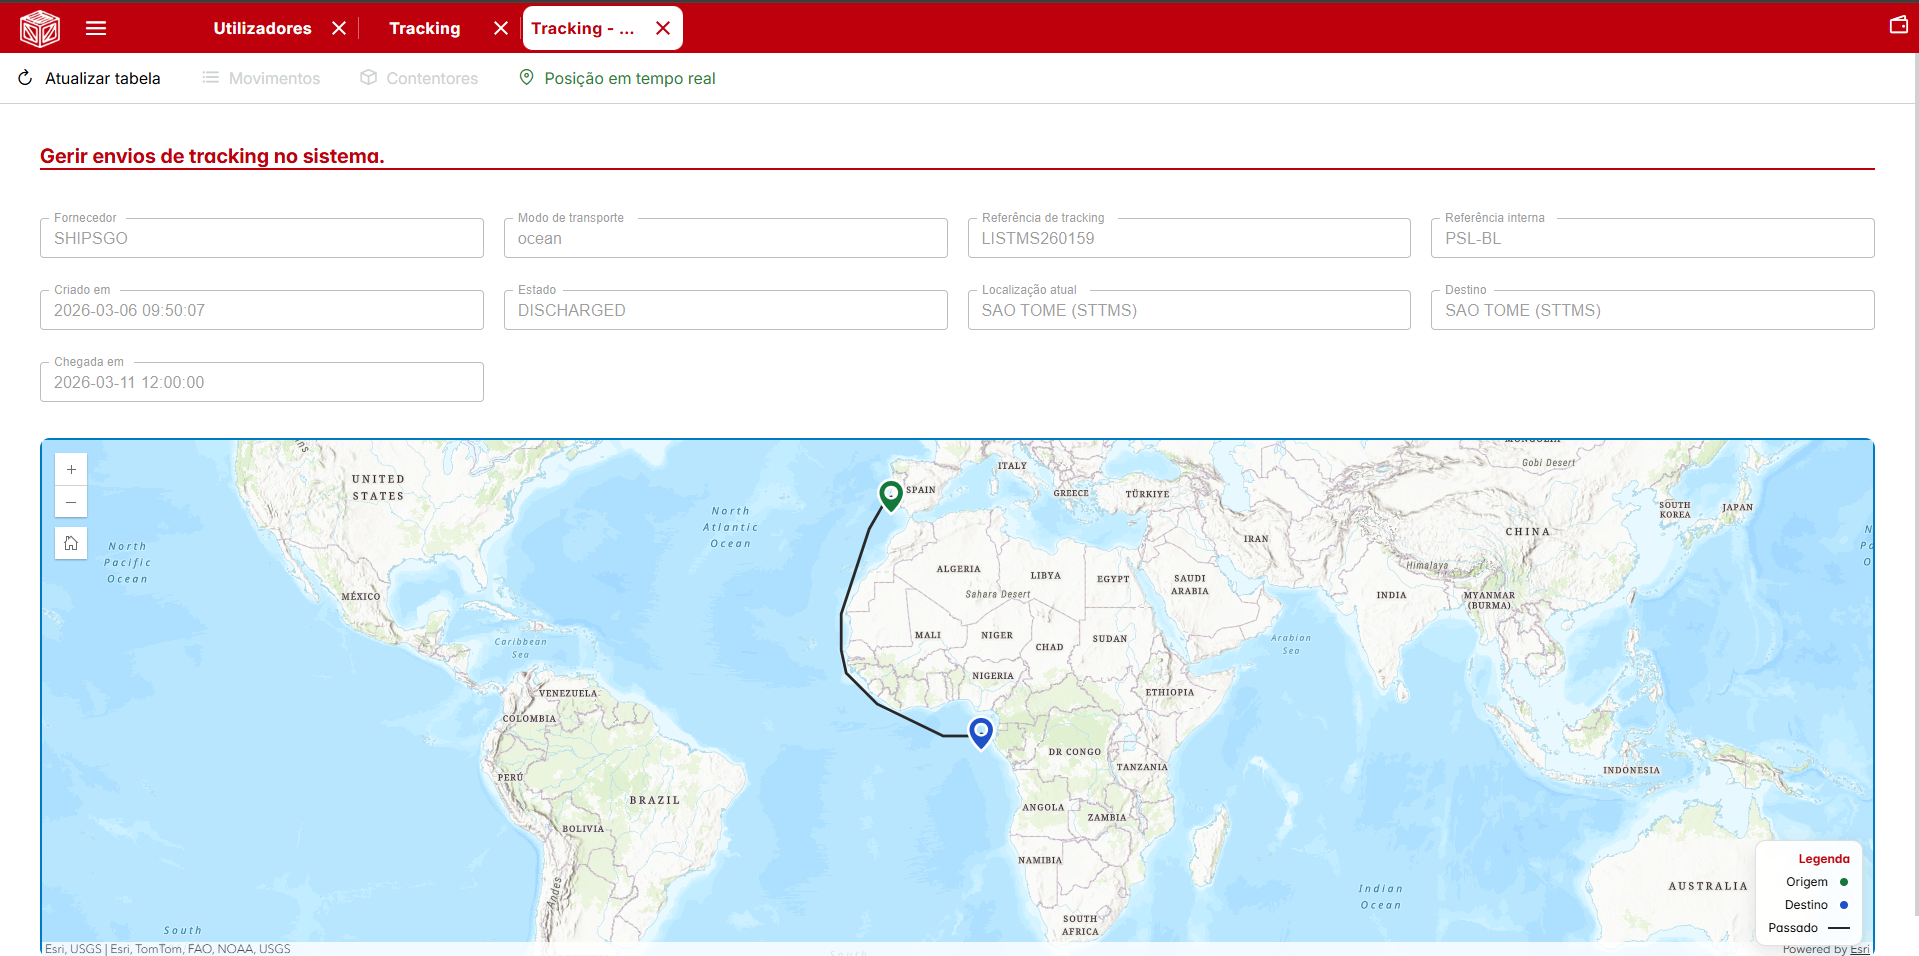
\includegraphics[width=\textwidth]{images/image20.png}
  \caption{Posição de envio finalizado}
  \label{fig:solucao-finalizado}
\end{figure}

\begin{figure}[H]
  \centering
  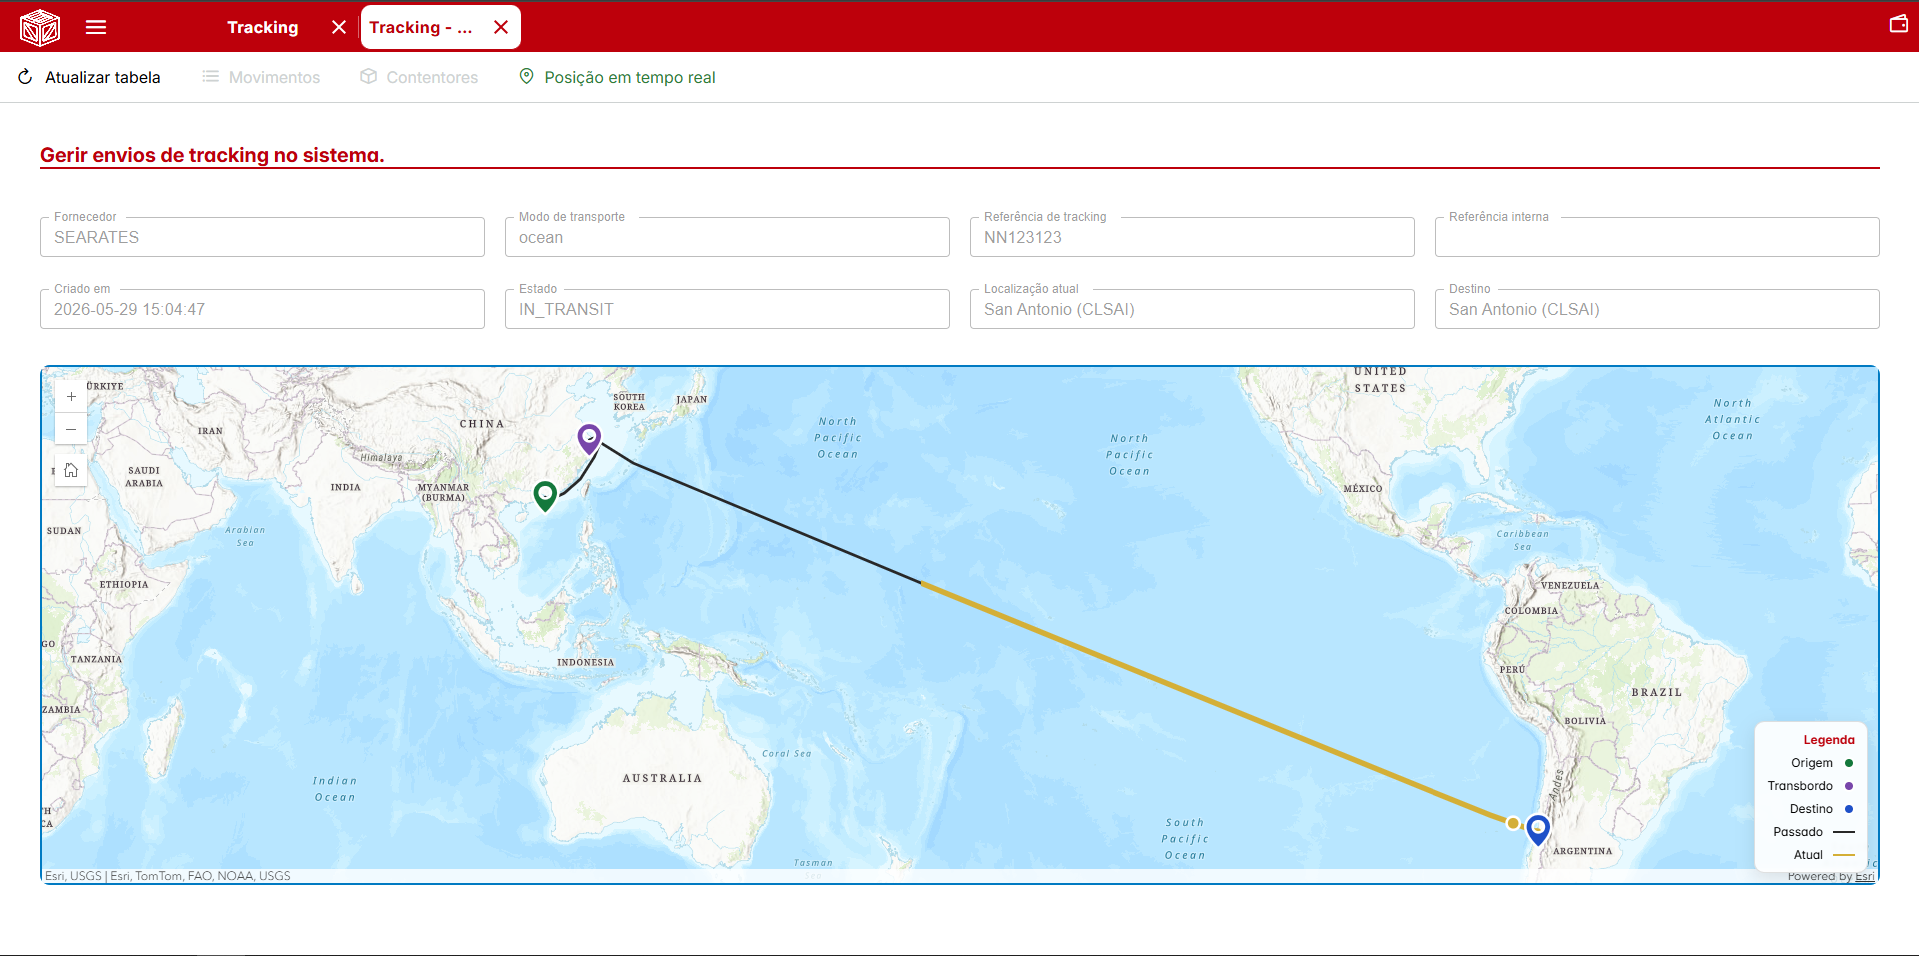
\includegraphics[width=\textwidth]{images/image21.png}
  \caption{Posição de envio em tempo real}
  \label{fig:solucao-temporeal}
\end{figure}

\begin{figure}[H]
  \centering
  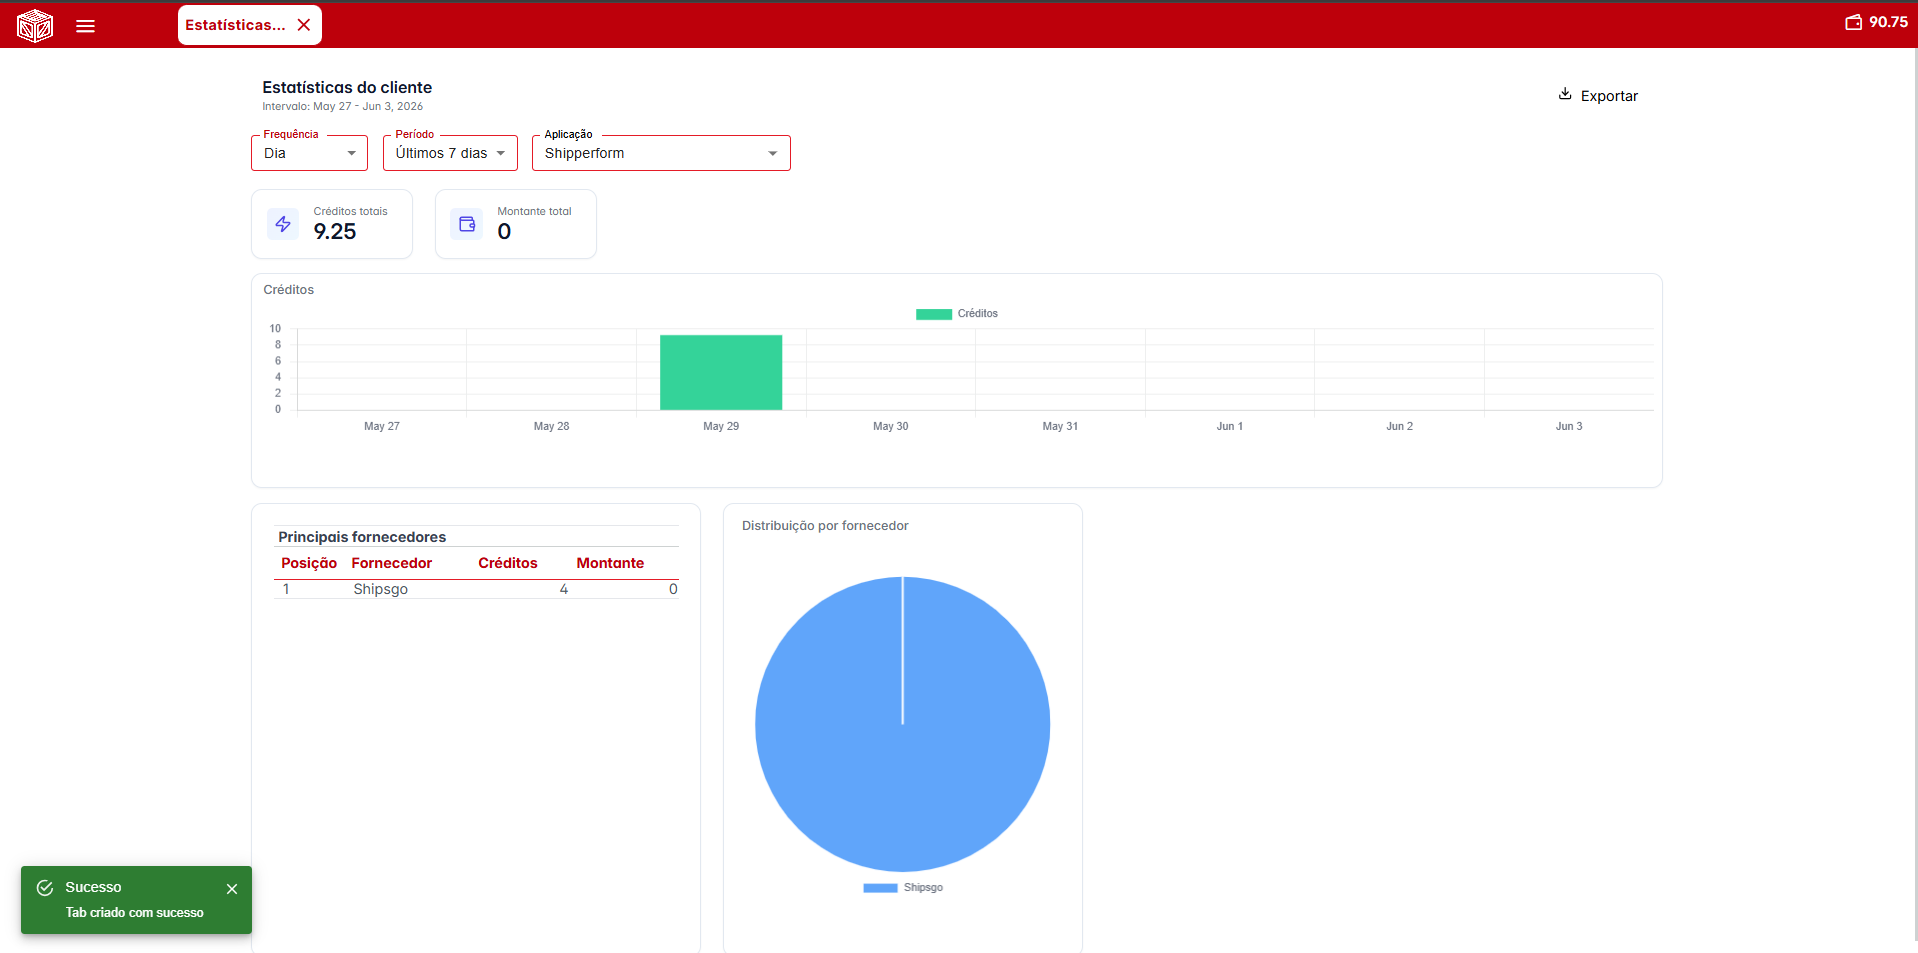
\includegraphics[width=\textwidth]{images/image22.png}
  \caption{Estatística do cliente}
  \label{fig:solucao-cliente}
\end{figure}

\begin{figure}[H]
  \centering
  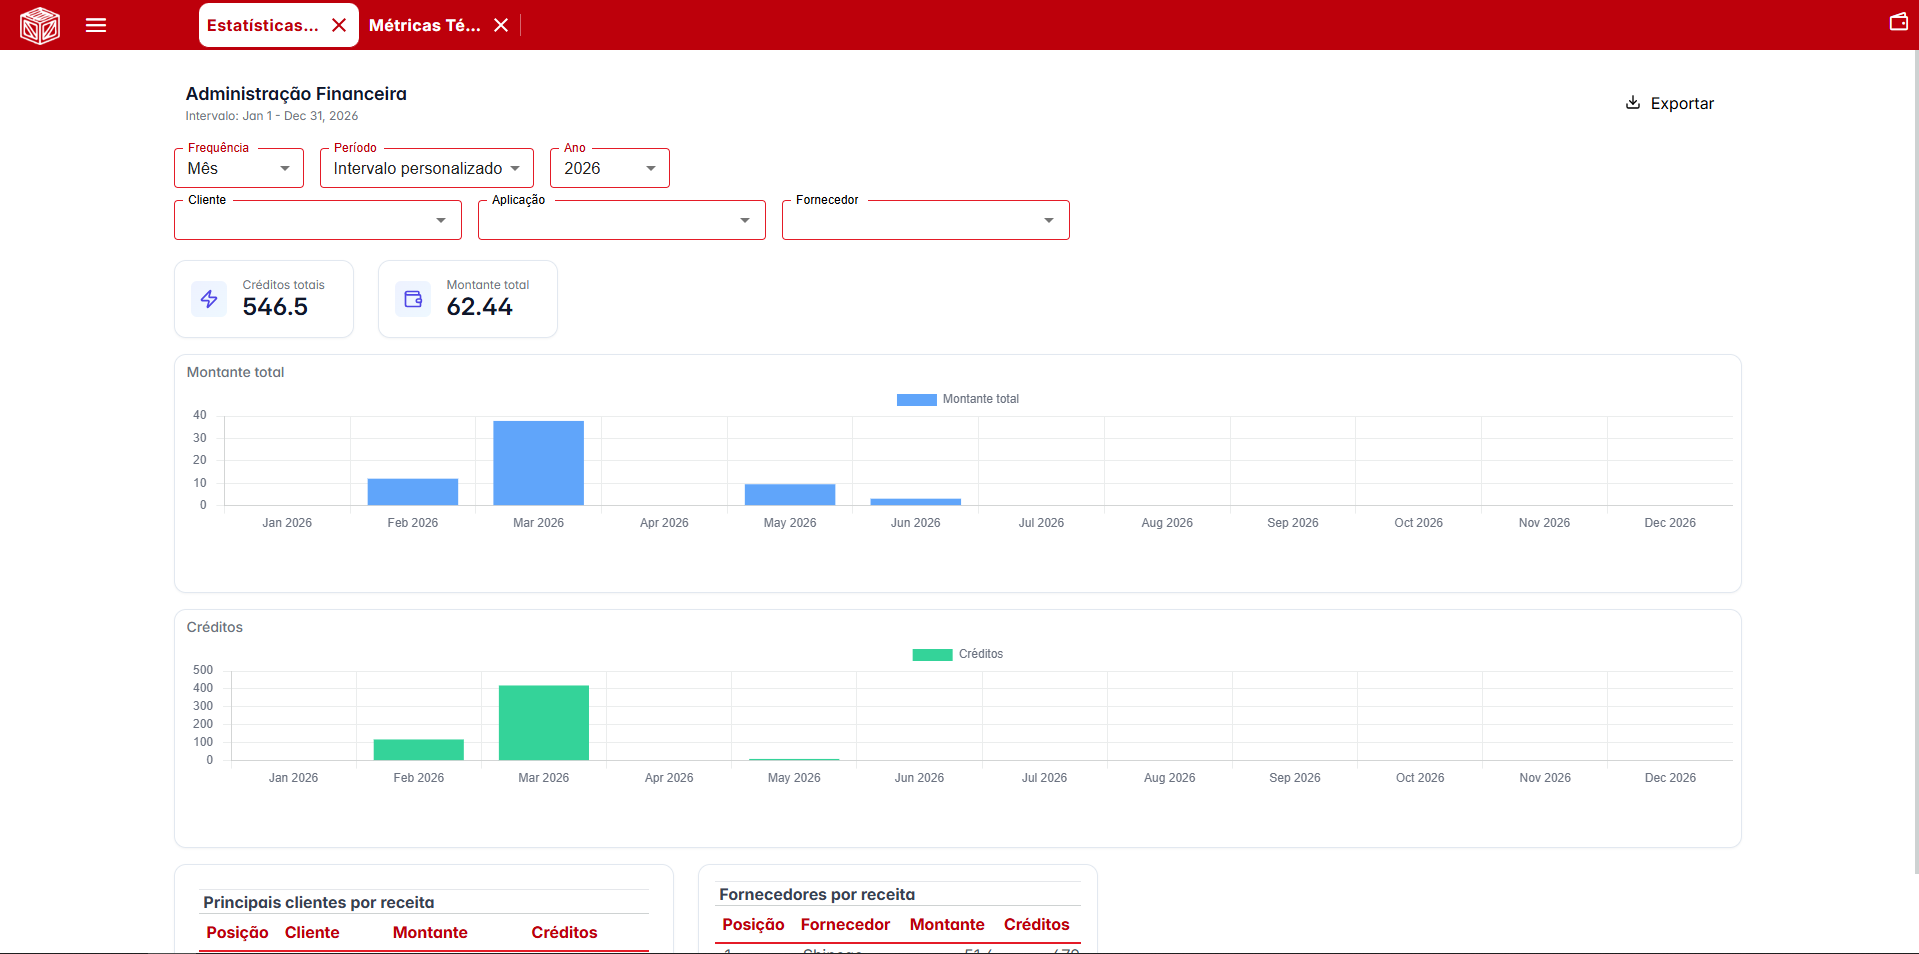
\includegraphics[width=\textwidth]{images/image23.png}
  \caption{Estatística financeira da plataforma}
  \label{fig:solucao-financeira}
\end{figure}

\begin{figure}[H]
  \centering
  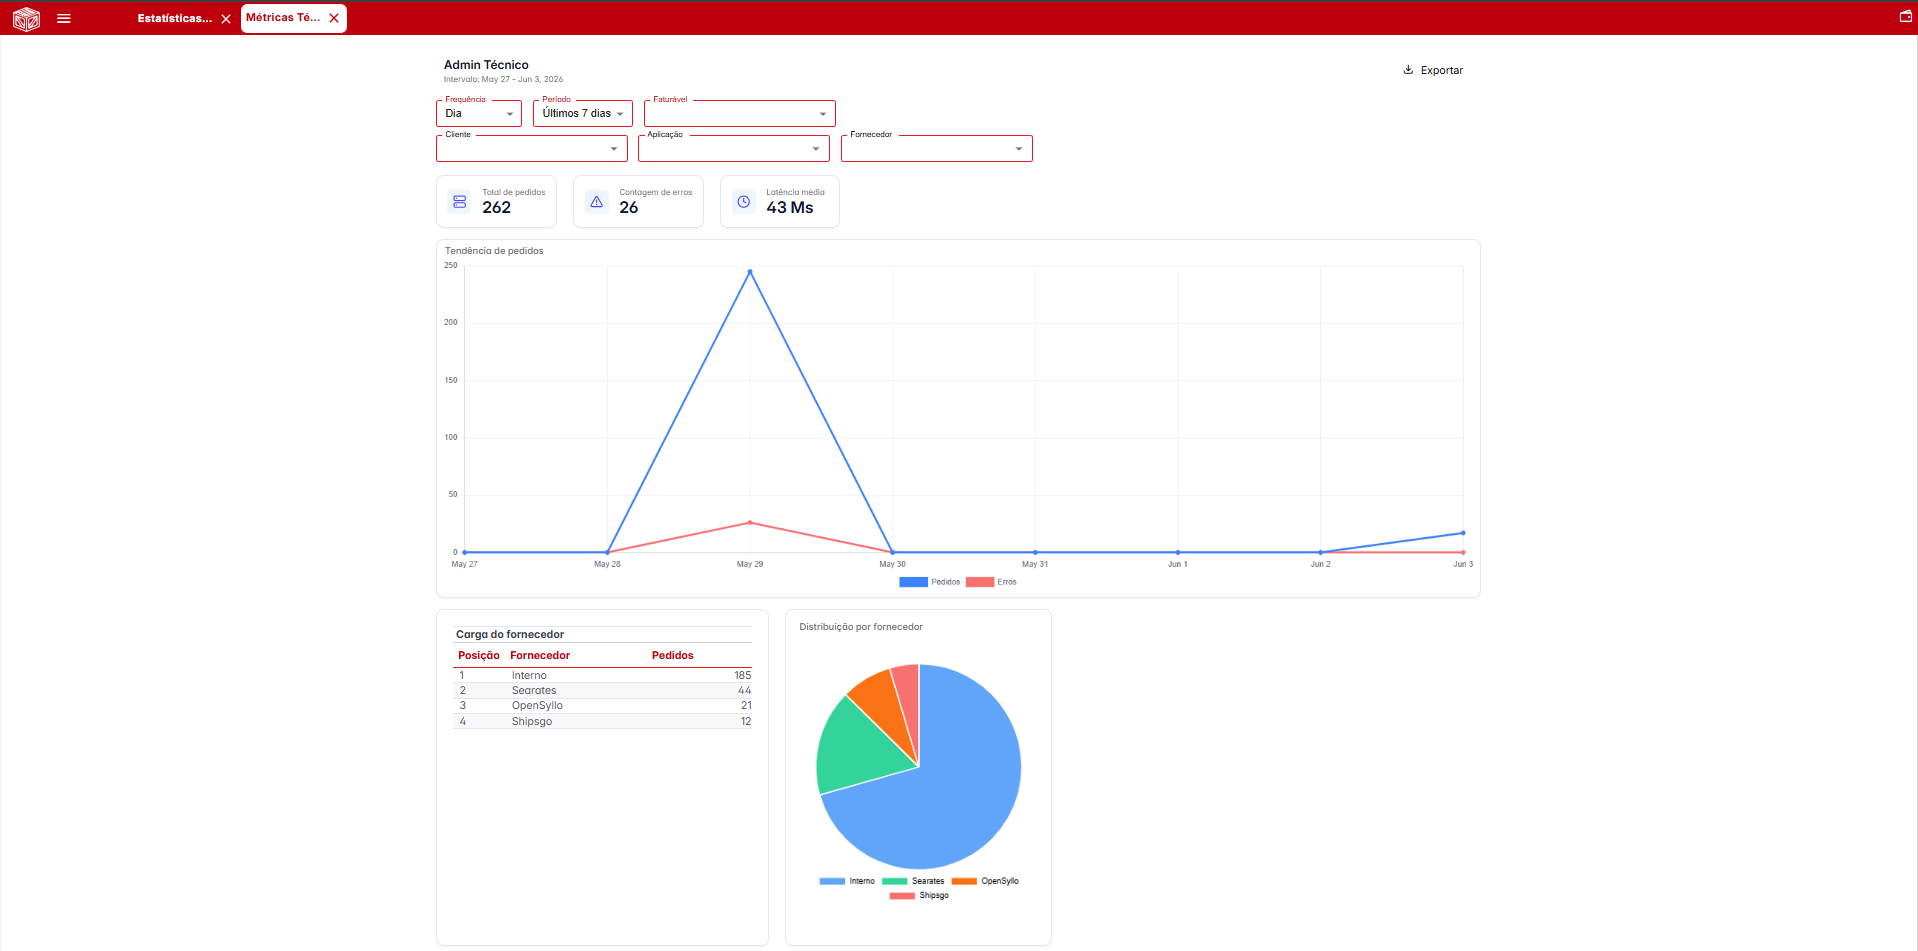
\includegraphics[width=\textwidth]{images/image24.png}
  \caption{Estatística técnica da plataforma}
  \label{fig:solucao-tecnica}
\end{figure}

% --- Anexo 8: Integração com a SeaRates (3 anexos) ---
\chapter{Integração com a \textit{SeaRates}}

\begin{figure}[H]
  \centering
  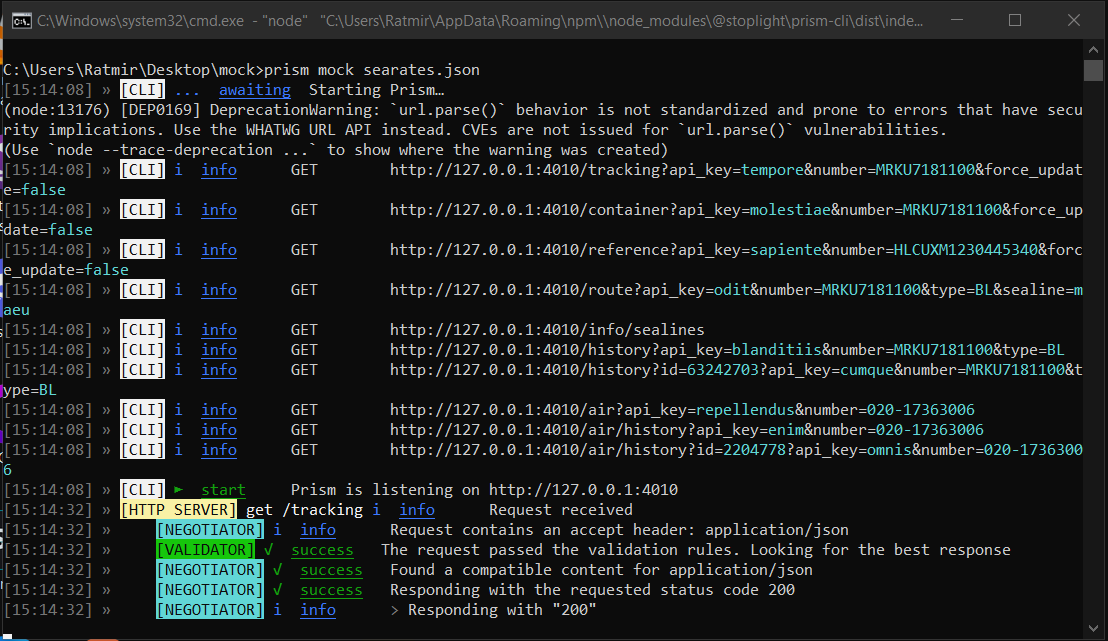
\includegraphics[width=\textwidth]{images/image25.png}
  \caption{Simulação da \textit{SeaRates} API com Prism}
  \label{fig:searates-prism}
\end{figure}

\begin{figure}[H]
  \centering
  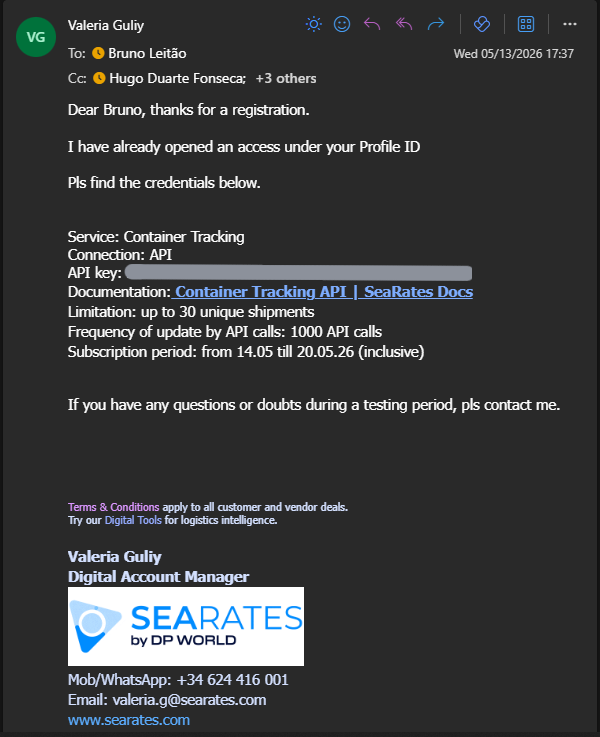
\includegraphics[width=\textwidth]{images/image26.png}
  \caption{Ativação do ambiente de teste da \textit{SeaRates}}
  \label{fig:searates-teste}
\end{figure}

\begin{figure}[H]
  \centering
  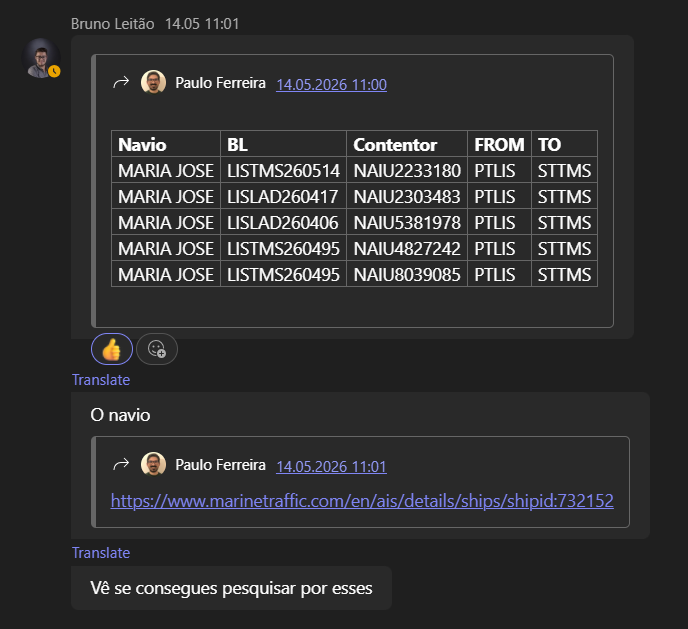
\includegraphics[width=\textwidth]{images/image27.png}
  \caption{Dados dos navios reais}
  \label{fig:searates-navios}
\end{figure}

\end{appendices}

\end{document}
